\documentclass[main]{subfiles}


\begin{document}
\newpage
\section{Unsupervised And Self-Supervised Learning}


\subsection{Introduction to Unsupervised Learning}
\subsubsection{Motivation}

Goeffrey Hinton (backprop\footnote{Learning representations by back-propagating errors}) suggests networks should be able to become intelligent on their own, unsupervised, without backprop.

\begin{enumerate}
    \item \textbf{Does not need labelled data.} In practice we often assume a fixed number of labels and call them cluster centers.
    \item \textbf {Is able to learn reveal the intricate structure (features) and can be used for dimensionality reduction.} This means we try to find projections in this this lower dimension space.
    \item Is able to generate new data examples that are consistent with the statistics of the training data.
    \item \textbf {Can predict future data examples (e.g. video frame prediction).} If we know the data representation we can try to find an inverse function out of our lower dimensional space. Which means we can sometimes reconstruct high dimensional data.
    \item \textbf {Can be used to detect familiar or out-of-distribution examples.} If we freeze our clusters, and then switch to another data set, then we can calculate the new data distance to the original data cluster centers.
    \item Can facilitate future supervised learning.
    \item Can be used to cluster the data.
    \item \textbf{Can be used to de-noise data.} We loose some information when projecting to a lower dimensional space. We optimize our method to retain the most useful information, this process might also de-noise our data.
    \item Can be used to encode data in a particular way (e.g. for data compression).
    \item We assume that humans have learned the world in an almost unsupervised way. 
\end{enumerate}

\begin{figure}[H]
	\centering
	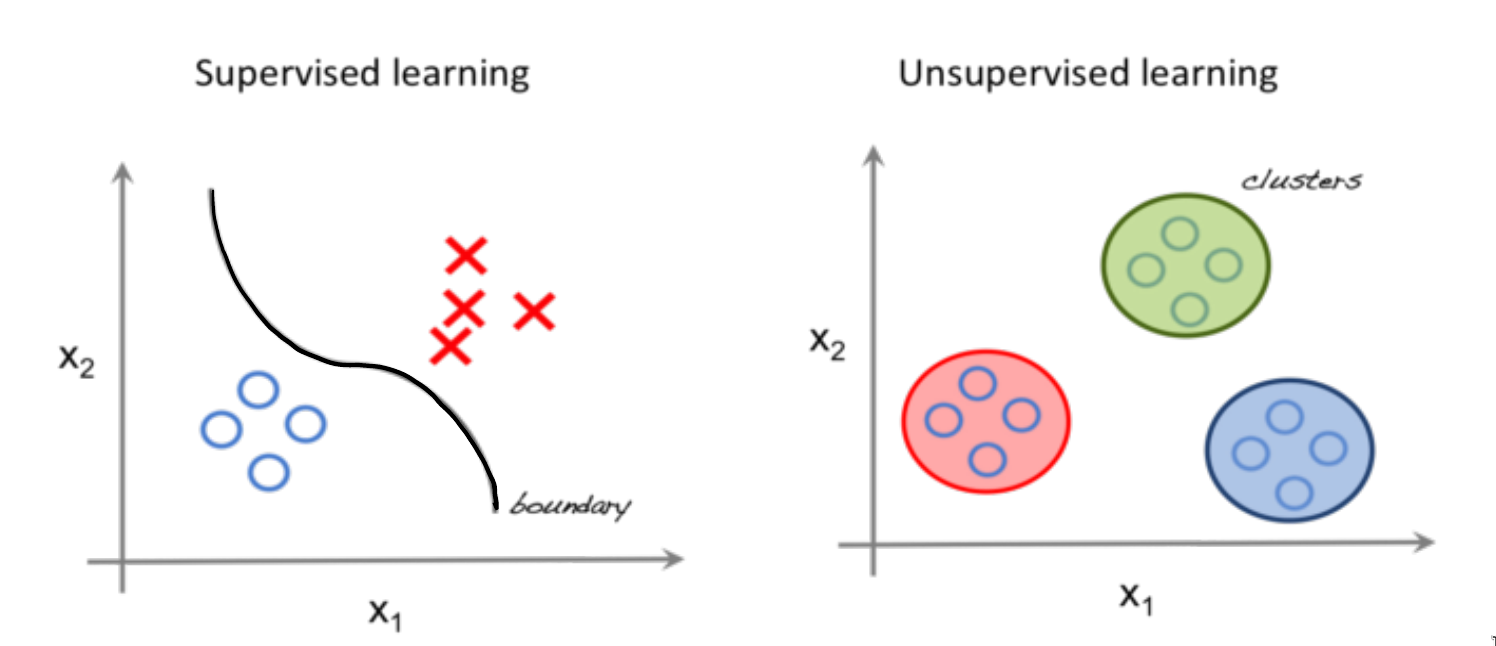
\includegraphics[width=0.99\linewidth]{07_UnsupervisedAndSelfsupervisedLearning/figures/sup-unsup-comp.png}
	\label{fig:sup-unsup-comp}
	\caption{The Difference between a supervised regression task where the data points are separated by some function that represents a bound in between different classes and an unsupervised clustering where the algorithm highlights the intrinsic structure of the data.}
\end{figure}

\subsubsection{Unsupervised Learning in the Brain}
We are aware of the fact that the brain as well uses unsupervised learning. Several examples were collected for the lecture.

In 1970 an experiment was conducted on cats. The kittens were housed from birth in a completely dark room, but form the age of 2 weeks they were put in a special apparatus for an average of about 5 hours a day. The kitten stood on a clear glass platform inside a tall cylinder of which the entire surface was covered in black and white stripes (in different experiments they used horizontal and vertical stripes). Those poor cats then were virtually blind for contours perpendicular to the orientation they had experienced. They recorded single neurons from primary visual cortex and found that almost all cats had their neurons trained to be most selective in direction of the stripes presented in the experiment. Example distribution in Figure \cref{fig:orientation-neurons}. \textbf{Interpretation: The neurons are the cluster centers and they move around during learning (growing up). When presented one stimulus only, then all cluster centers group in the same optimum.}

\begin{figure}[H]
	\centering
	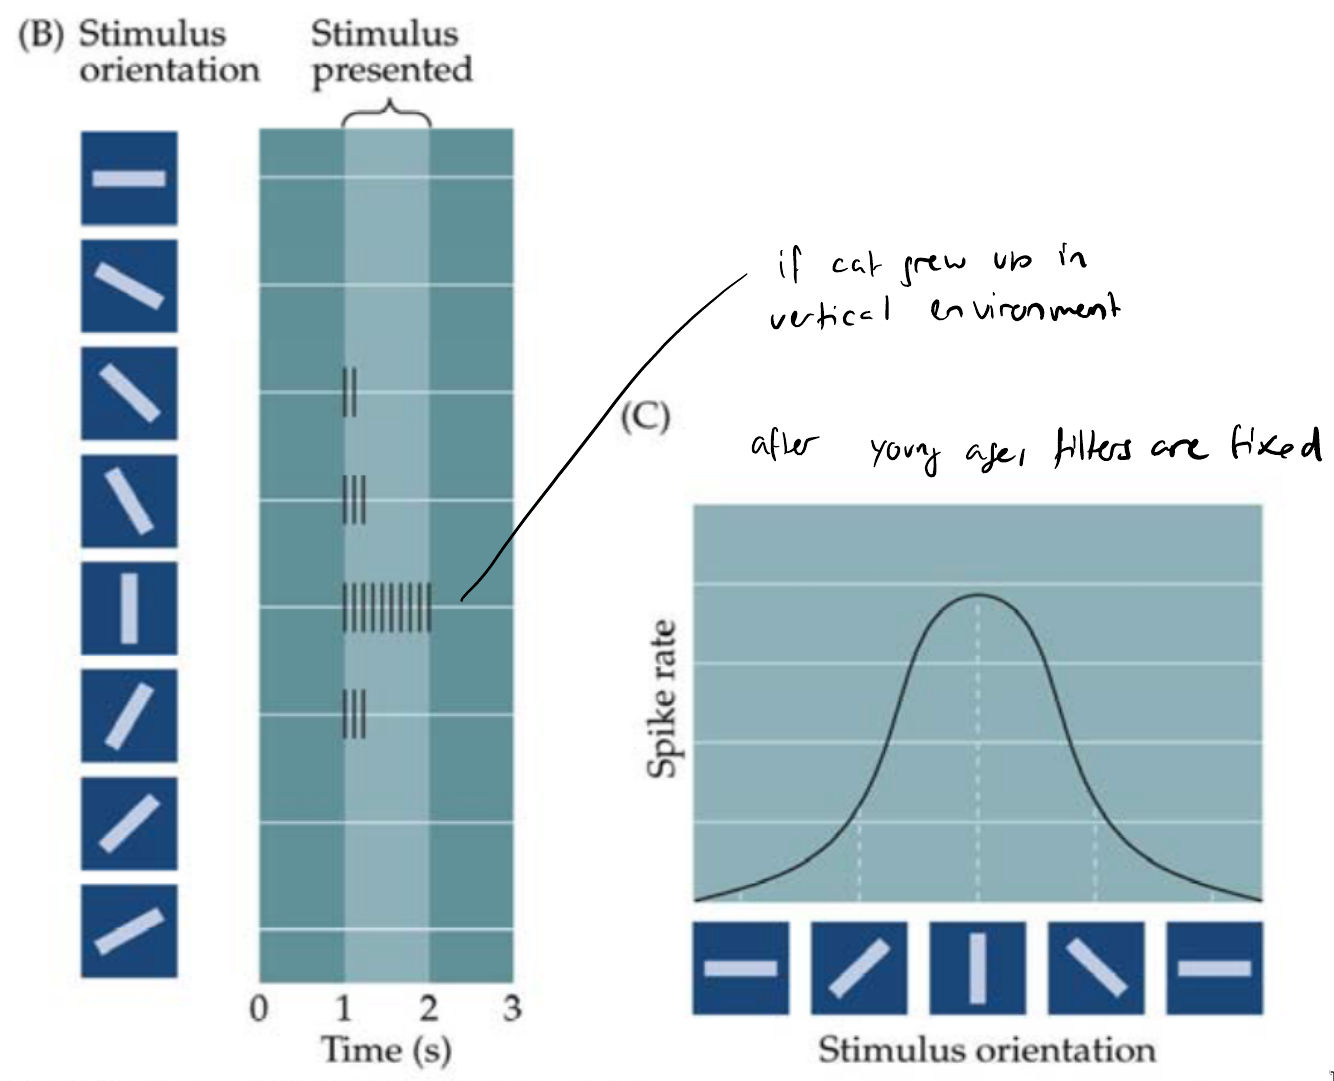
\includegraphics[width=0.5\linewidth]{07_UnsupervisedAndSelfsupervisedLearning/figures/orientation-neurons.png}
	\label{fig:orientation-neurons}
	\caption{A spike rate curve of a single neuron with respect to the neurons orientation. Experiments show that this distribution changes in adolescent subjects and becomes more rigid with increasing age.}
\end{figure}

Another group analyzed visual cortical activity of awake ferrets during development (2007). They provide and one-sentence summary: The relation between spontaneous activity and activity evoked by natural stimuli in the primary visual cortex reveals that the cortical circuit progressively adapts its internal model to the statistical structure of the environment. \footnote{Spontaneous Cortical Activity Reveals Hallmarks of an Optimal
Internal Model of the Environment}

\begin{figure}[H]
	\centering
	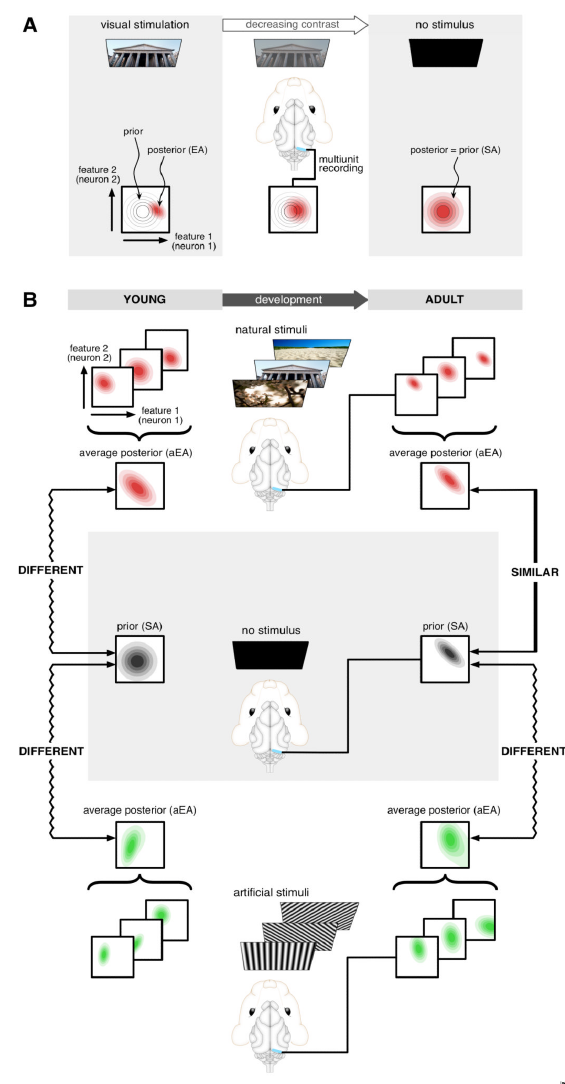
\includegraphics[width=0.7\linewidth]{07_UnsupervisedAndSelfsupervisedLearning/figures/ferret.png}
	\label{fig:ferret}
	\caption {Notation: Evoked and spontaneous (dark) neural activity (EA and SA). Multi-neural EA (aEA) \textbf{(A)} The posterior distribution represented by EA is increasingly dominated by the prior distribution as brightness or contrast is decreased. \textbf{(B)} ferrets either receiving no stimulus (middle) or viewing natural (top) or artificial stimuli (bottom) is used to construct neural activity distributions in young and adult animals. It reveals the level of statistical adaptation of the internal model to the stimulus ensemble. The internal model of young animals (left) is expected to show little adaptation to the natural environment and thus aEA for natural (and also for artificial) scenes should be different from SA. Adult animals (right) are expected to have adapted to natural scenes and thus to exhibit a high degree of similarity between SA and natural stimuli aEA, but not between SA and artificial stimuli aEA.}
\end{figure}


We now know that these distributions adapt, but from the presented experiments it's unclear what the conditions are to trigger an adaption. Another experiment \footnote{Stimulus Timing-Dependent Plasticity in Cortical Processing of Orientation} shows that the  relative  timing  of  presynaptic  and  postsynaptic spikes plays a critical role in activity-induced synaptic orientation (single unit recording in cat V1). Induction of a significant shift required that the interval between the pair fall within +-40 ms otherwise nothing changed.

Another path to understand the learning in neural circuits leads to the recent advances in deep neural networks (DNN). Several groups tried to map layers (as in DNN layers) to cortical regions. Several mapping strategies were found. We can show that dissimilarity matrices of regions in both system look similar, especially in higher cortical regions vs deeper layers of neural networks. Interestingly, the animals we recorded from never knew any labels that were used to train the DNNs.

\begin{figure}[H]
	\centering
	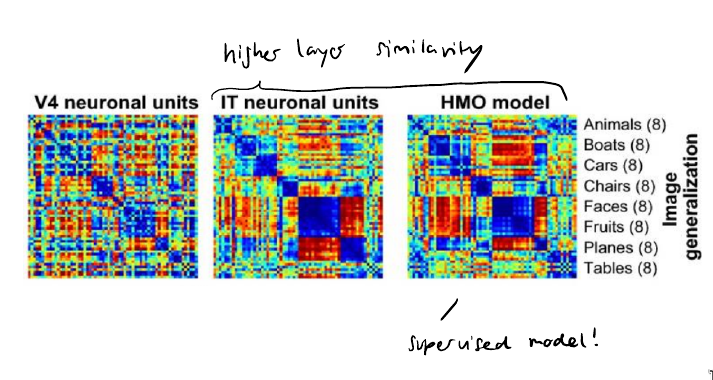
\includegraphics[width=0.9\linewidth]{07_UnsupervisedAndSelfsupervisedLearning/figures/conf-matrix.png}
	\label{fig:conf-matrix}
	\caption{Confusion Matrix of V4 neural units and units in artificial networks from a comparable depth.}
\end{figure}


\subsection{Sparse Coding}
The sparse code is found when each sample of a given data set is encoded by the strong activation of a relatively small set of neurons. For each item to be encoded, this is a different subset of all available neurons. 

Each image can be represented by a set of basis functions:

\begin{equation}
    I(x,y) \approx \sum_i a_i \phi_i(x,y) = \hat{I}
\end{equation}

We define an energy function which is essentially true image $I$ minus approximation $\tilde{I}$ + regularizer $S$:

\begin{equation}
    E = \sum_{x,y}[I(x,y)-\sum_i a_i  \phi_i(x,y)]^2 + \lambda \sum_i S(\frac{a_i}{\tau})
\end{equation}

Presented in the lectures was a set of known regularizers $\mathbb{S}$:

\begin{equation}
    S \in \mathbb{S} = \{ \exp^{x^2}, log(1+x^2), \|x\| \}
\end{equation}

For each image presentation $E$ is mimized with respect to $a_i$.
The $a_i$ are determined by the equilibrium solution of the differential equation (the paper does not show a proof):

\begin{equation}
    \frac{\partial E}{\partial a_i} = \Dot{a_i} = b_i - \sum_j c_{ij}a_j - \frac{\lambda} {\tau} S'(\frac{a_i}{\tau})
\end{equation}

\begin{equation}
    b_i = \sum_{x,y} \phi_i(x,y)I(x,y)
\end{equation}
    
\begin{equation}
    c_{ij} = \sum_{x,y} \phi_i(x,y)\phi_j(x,y)
\end{equation}

The $\phi_i$ then evolve by gradient descent on $E$ averaged over many image presentations. The learning rule for updating $\phi$ is then:

\begin{equation}
    \nabla \phi_i(x_m, y_n) = \eta \langle a_i [I(x_m, y_n) - \hat{I}(x_m, y_n)] \rangle
\end{equation}

Comments on Parameters and Operations:
\begin{itemize}
    \item $a_i$ factors, should be sparse, different for each sample
    \item $\phi$ components, basis functions that are the same over all samples
    \item $\tau$ scaling constant
    \item $\lambda$ scaling constant: sparseness vs information perseverance
    \item $\eta$ learning rate
    \item $\langle x \rangle$ mean
\end{itemize}

\begin{figure}[H]
	\centering
	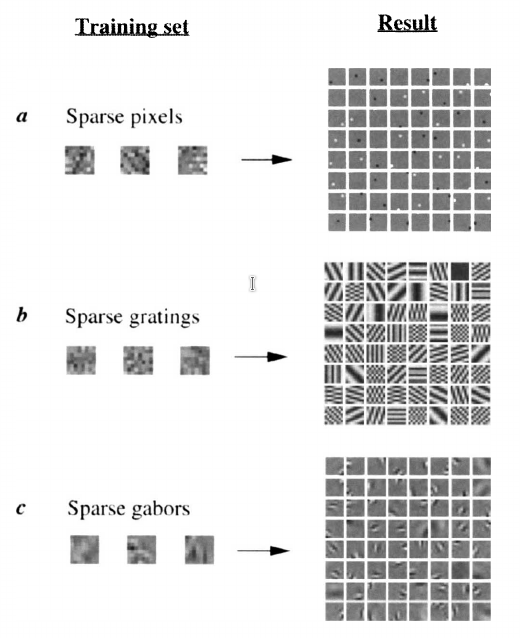
\includegraphics[width=0.5\linewidth]{07_UnsupervisedAndSelfsupervisedLearning/figures/sparse-coding-filters.png}
	\label{fig:sparse-coding-filters}
	\caption{Training examples and the respective basis functions of sparse coding.}
\end{figure}

\subsubsection{Relation to Neuroscience}
The paper \footnote{Spatial structure of neuronal receptive field in awake monkey secondary visual cortex} shows that cells of sub-units in V1 have receptive fields that apply signal filtering that is very similar to sparse coding. In V2 they identified sub-units with spatial feature selectivity.

\begin{figure}[H]
	\centering
	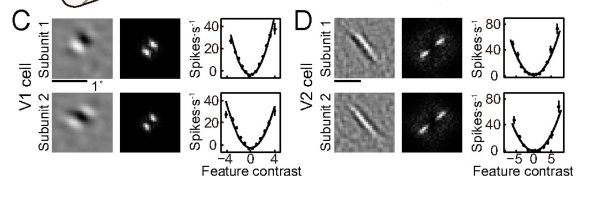
\includegraphics[width=0.5\linewidth]{07_UnsupervisedAndSelfsupervisedLearning/figures/sparse-coding-brain.png}
	\label{fig:sparse-coding-brain}
	\caption{Sparse coding in the brain.}
\end{figure}


\subsection{Infomax (ICA)}
Infomax is an optimization principle for artificial neural networks and other information processing systems. It prescribes that a function that maps a set of input values I to a set of output values O should be chosen or learned so as to maximize the average Shannon mutual information between I and O. One of the applications of Infomax has been to an independent component analysis algorithm (ICA) that finds independent signals by maximizing entropy. ICA via mutual information is one way to find independent components.

The independence criterion is stronger than uncorrelatedness which is defined as:
\begin{equation}
    \langle X_1 X_2 \rangle - \langle X_2 \rangle \langle X_1 \rangle = 0
\end{equation}
or 
\begin{equation}
   Cov(X_1, X_2) = \textbf{E}[X_1 X_2] - \textbf{E}[X_1]\textbf{E}[X_2] = 0
\end{equation}
Remember: If two variables are uncorrelated, there is no linear relationship between them. However this does not mean that they are independent. The other way works: if $X_1$ and $X_2$ are independent (with finite second moments), then they are uncorrelated.

For ICA we want statistical independence

\begin{equation}
    p(\alpha_{1:N}) = \prod_{i=1}^N p(\alpha_i)
\end{equation}

To measure the degree of dependence we look at the pairwise mutual information of two random variables $X$, $Y$. Mutual information is non-negative and symmetric:

\begin{align}
  \operatorname{I}(X;Y) &{} \equiv H(X) - H(X|Y) \\
     &{} \equiv H(Y) - H(Y|X) \\
     &{} \equiv H(X) + H(Y) - H(X, Y) \\
     &{} \equiv H(X, Y) - H(X|Y) - H(Y|X) \\
    I(X;Y)& = D_{\mathrm{KL}}( P_{(X,Y)} \| P_{X} \otimes P_{Y} )
\end{align}

We use the entropy:
\begin{equation}
    H(X) = -\sum_{i=1}^n {\mathrm{P}(x_i) \log_b \mathrm{P}(x_i)}
\end{equation}

Idea: $X$, $Y$ independent if:
\begin{equation}
 p(X, Y) = p(X)p(Y)
\end{equation}

For the discrete case we can then see best that last part of eq. is $log(1) = 0$:

\begin{equation}
    \operatorname{I}(X;Y) = \sum_{y \in \mathcal Y} \sum_{x \in \mathcal X}
    { p_{(X,Y)}(x,y) \log{ \left(\frac{p_{(X,Y)}(x,y)}{p_X(x)\,p_Y(y)} \right) }},
\end{equation}


\begin{figure}[H]
	\centering
	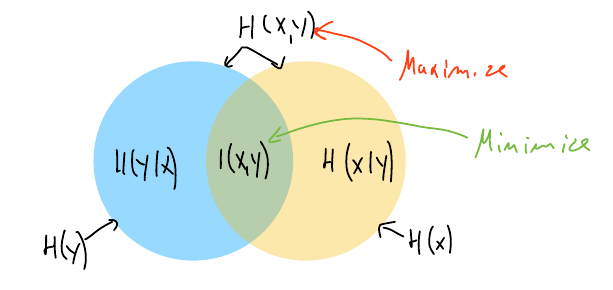
\includegraphics[width=0.8\linewidth]{07_UnsupervisedAndSelfsupervisedLearning/figures/mutual-info.png}
	\label{fig:mutual-info}
	\caption{Venn diagram of the Infomax objective: We want to maximize the entropy and minimize the mutual information. Entropy maximization forces the network to generalize. See: principle of maximum entropy.}
\end{figure}

How do we actually implement Infomax? We can think of Infomax as a one layer linear neural network that produces
\begin{equation}
\textbf{y} = \textbf{W}\textbf{x}
\end{equation}
such that outputs $y_i$ are maximally independent:

\begin{equation}
\forall (y_i, y_j), i\neq j,  y_i,y_j \in \textbf{y}: I(y_i, y_j) = I_{min}
\end{equation}
but keep in mind we also maximize $I(X;Y)$. In the lecture, $\textbf{y}$ somehow converges to a set of Gabor-like filters, but it was not specified in detail why.If somebody knows, please contact me (RT).

\begin{figure}[H]
	\centering
	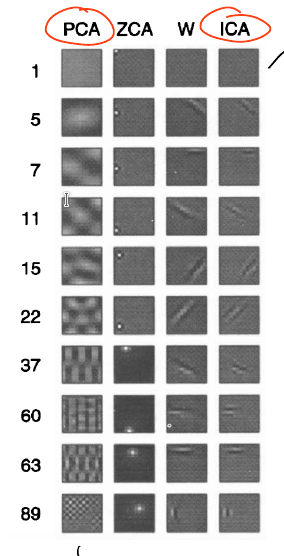
\includegraphics[angle=90,width=0.8\linewidth]{07_UnsupervisedAndSelfsupervisedLearning/figures/ica-filters.png}
	\label{fig:ica-filters}
	\caption{We can see that the PCA features are very different from what we know that the brain uses for feature representation. However the ICA representation looks like the (Gabor-like) filters from the previous chapter.}
\end{figure}

\begin{itemize}
    \item ICA is similar to Principal Component Analysis, except that we’re looking for a transformation subject to the stronger requirement of independence, rather than uncorrelatedness.
    \item In general, no analytic solution (like eigenvalue decomposition for PCA) exists. Thus, ICA is typically implemented using neural network models and GD.
    \item For the ICA NN implementation, we need an architecture and an objective function to descend/climb.
    \item Results in N independent (or as independent as possible) components in an N-dimensional space; these don’t need need to be orthogonal (PCA is an orthogonal transformation).
\end{itemize}


\subsection{Autoencoders}

\begin{figure}[H]
	\centering
	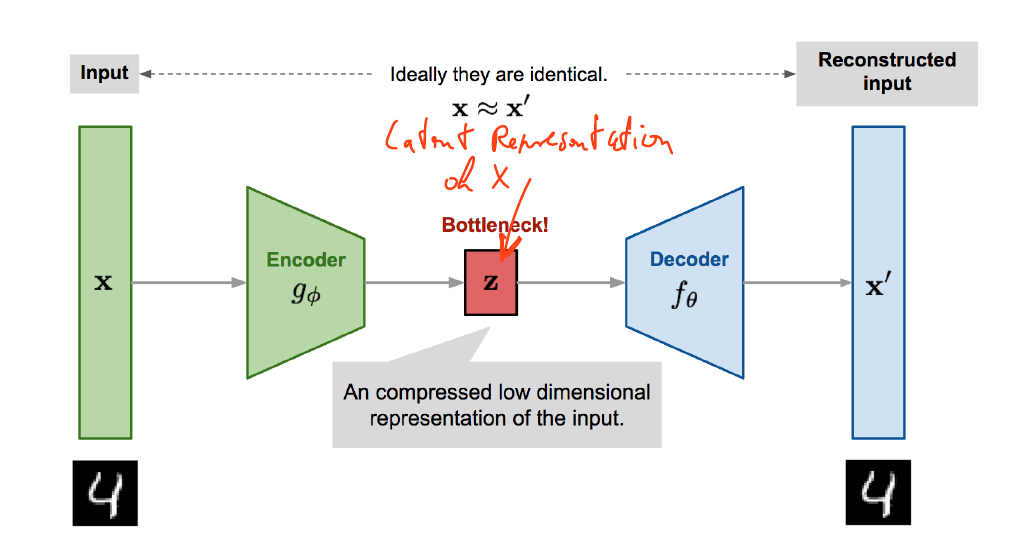
\includegraphics[width=0.8\linewidth]{07_UnsupervisedAndSelfsupervisedLearning/figures/autoencoder.png}
	\label{fig:autoencoder}
	\caption{Autoencoder}
\end{figure}

Autoencoder loss function:

\begin{equation}
    L_{AE} = \frac{1}{2} \| \textbf{x} - \textbf{x'} \|^2, \textbf{x'} = f_\theta(g_\phi(\textbf{x}))
\end{equation}

The autoencoder is trained by gradient descent.

Comments on Parameters and Operations:
\begin{itemize}
    \item $\phi$ parameters of encoding function (trainable)
    \item $\theta$ parameters of decoding function (trainable)
    \item $g_\phi$ encoding function 
    \item $f_\theta$ decoding function
\end{itemize}

\subsubsection{Semi-supervised autoencoder}
The supervised AE uses the latent space to define a second decoding pathway. This path is added as another term to the loss and one calculates the gradients from two different ends. In the shared part, these gradients then merge. This is called multi-task learning (having a shared pathway for different objectives).

\begin{equation}
    L_{SAE} = \frac{1}{t} \sum_{i=1}^t [L_p(\mathbf{x_i}, \mathbf{W}_{1:2}, \mathbf{y_i}) + L_v(\mathbf{x_i}, \mathbf{W}_{1:4}, \hat{\mathbf{x}}_i)]
\end{equation}

\begin{itemize}
    \item $L_p$ loss of label $y_i$
    \item $L_v$ loss of reconstruction $\hat{x_i}$
    \item $W_{1,2}$ weights of encoder (that produce label $y$)
    \item $W_{1,4}$ weights of encoder + decoder
\end{itemize}

\begin{figure}[H]
	\centering
	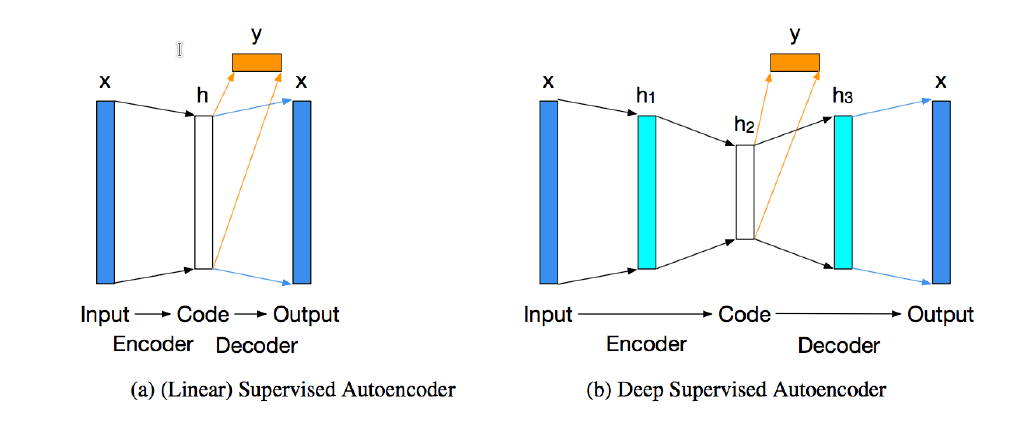
\includegraphics[width=0.8\linewidth]{07_UnsupervisedAndSelfsupervisedLearning/figures/autoencoder-semi.png}
	\label{fig:autoencoder-semi}
	\caption{Semi-supervised autoencoder}
\end{figure}

\subsubsection{De-noising Autoencoder}
Since the autoencoder learns the identity function, we are facing the risk of “overfitting” when there are more network parameters than the number of data points. To avoid overfitting and improve the robustness, Denoising Autoencoder (Vincent et al. 2008) proposed a modification to the basic autoencoder. The input is partially corrupted by adding noises to or masking some values of the input vector in a stochastic manner. To “repair” the partially destroyed input, the denoising autoencoder has to discover and capture relationship between dimensions of input in order to infer missing pieces. Similar to dropout.

\begin{align}
\tilde{\mathbf{x}}^{(i)} &\sim \mathcal{M}_\mathcal{D}(\tilde{\mathbf{x}}^{(i)} \vert \mathbf{x}^{(i)})\\
L_\text{DAE}(\theta, \phi) &= \frac{1}{n} \sum_{i=1}^n (\mathbf{x}^{(i)} - f_\theta(g_\phi(\tilde{\mathbf{x}}^{(i)})))^2
\end{align}

\begin{figure}[H]
	\centering
	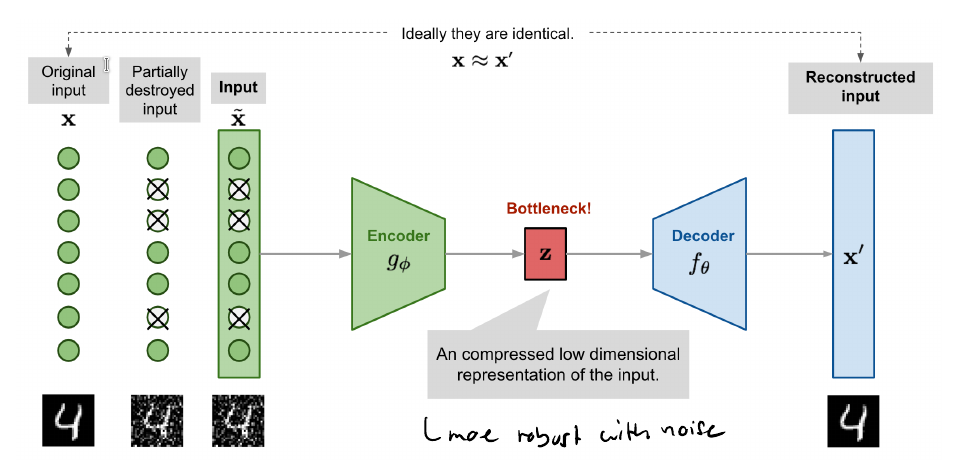
\includegraphics[width=0.8\linewidth]{07_UnsupervisedAndSelfsupervisedLearning/figures/autoencoder-denoise.png}
	\label{fig:autoencoder-denoise}
	\caption{De-noising autoencoder}
\end{figure}

\subsubsection{Sparse Autoencoder}
The Sparse Autoencoder applies a sparsity constraint on the hidden unit activation to avoid overfitting and improve robustness. It forces the model to only have a small number of hidden units being activated at the same time.
\begin{equation}
    \hat{\rho}_j^{(l)} = \frac{1}{n} \sum_{i=1}^n [a_j^{(l)}(\mathbf{x}^{(i)})] \approx \rho
\end{equation}

Let’s say there are $s_l$ neurons in the $l$-th hidden layer and the activation function for the $j$-th neuron in this layer is labelled as $a^{(l)}_j(.)$, $j=1,…,s_l.$ The fraction of activation of this neuron $\rho^j$ is expected to be a small number $\rho$, known as sparsity parameter; a common config is $\rho=0.05$. 

\begin{align}
L_\text{SAE}(\theta) 
&= L(\theta) + \beta \sum_{l=1}^L \sum_{j=1}^{s_l} D_\text{KL}(\rho \| \hat{\rho}_j^{(l)}) \\
&= L(\theta) + \beta \sum_{l=1}^L \sum_{j=1}^{s_l} \rho\log\frac{\rho}{\hat{\rho}_j^{(l)}} + (1-\rho)\log\frac{1-\rho}{1-\hat{\rho}_j^{(l)}}
\end{align}

Keep in mind that we specify our desired target distribution that is $\rho$. Common activation functions include sigmoid, tanh, relu, leaky relu, etc. 

\subsubsection{Contracting Autoencoder}
Similar to sparse autoencoder, Contractive Autoencoder (Rifai, et al, 2011) encourages the learned representation to stay in a contractive space for better robustness.

It adds a term in the loss function to penalize the representation being too sensitive to the input, and thus improve the robustness to small perturbations around the training data points. The sensitivity is measured by the Frobenius norm of the Jacobian matrix of the encoder activations with respect to the input:

\begin{equation}
    \|J_f(\mathbf{x})\|_F^2 = \sum_{ij} \Big( \frac{\partial h_j(\mathbf{x})}{\partial x_i} \Big)^2
\end{equation}

where $h_j$ is one unit output in the compressed code $\mathbf{z} = f(x)$.

This penalty term is the sum of squares of all partial derivatives of the learned encoding with respect to input dimensions. The authors claimed that empirically this penalty was found to carve a representation that corresponds to a lower-dimensional non-linear manifold, while staying more invariant to majority directions orthogonal to the manifold.\footnote{\url{https://lilianweng.github.io/lil-log/2018/08/12/from-autoencoder-to-beta-vae.html#sparse-autoencoder}}
\subsection{Competitive Learning}
Competitive learning is a form of unsupervised learning in artificial neural networks, in which nodes compete for the right to respond to a subset of the input data. A variant of Hebbian learning, competitive learning works by increasing the specialization of each node in the network. It is well suited to finding clusters within data. Imagine that we move our neuron around that space by adjusting the weights.

\begin{itemize}
    \item Neurons/Nodes are all the same except for their weights.
    \item A competitive mechanism permits neurons to compete for the right to respond to a given subset of inputs, such that only one output neuron (or only one neuron per group), is active (i.e. "on") at a time.
    \item The neuron that wins the competition is called a "winner-take-all" neuron and is allowed to update it’s weights.
    \item During ‘learning’ individual neurons of the network learn to specialize on ensembles of similar patterns and become 'feature detectors' for different classes of input patterns.
    \item The competitive networks are able to recode sets of correlated inputs to a few output neurons.
\end{itemize}

\subsubsection{The CL Algorithm}
The competitive learning algorithm (two clusters):
\begin{enumerate}
    \item Let all inputs feed into two different nodes, so that every hidden node is connected to every input. Initialize the weights randomly between 0.0 and 1.0. Calculate the activity of each hidden node for the first input.
    \item The hidden node with the highest output is the winner for the cluster to which the data point belongs.
    \item The winner node updates each of its weights, thereby moving its weight vector towards the data point.
    \item Repeat with the next data point.
\end{enumerate}

\begin{figure}[H]
	\centering
	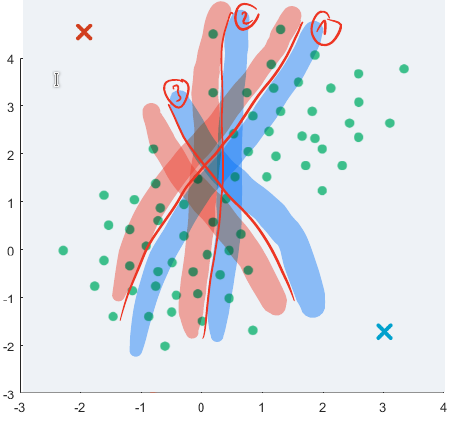
\includegraphics[width=0.5\linewidth]{07_UnsupervisedAndSelfsupervisedLearning/figures/competitive-barrier.png}
	\label{fig:competitive-barrier}
	\caption{Illustration of how the barrier would move if the blue neuron would move upwards in direction of the cluster center and the red one downwards (3 iterations are shown). However after revisiting this example I think the blue one would occupy the lower cluster!}
\end{figure}

\subsection{CL with Neural Networks}

We ask for the neuron with the closest weight vector:
\begin{align} 
    \| u-w_i \| &= u^Tu - 2 w_i^Tu + w_i^Tw_i = \| u \|^2 + \| w_i \|^2 - 2y_i \\
    argmin \| u-w_i \| &= argmax (y_i)
\end{align}

We update our weights accordingly:
\begin{align} 
    w_A(t) &= \frac{1}{t}\sum_{o=1}^t u_t \\
    \nabla w_A &= \eta (u_t - w_A)
\end{align}

\begin{figure}[H]
	\centering
	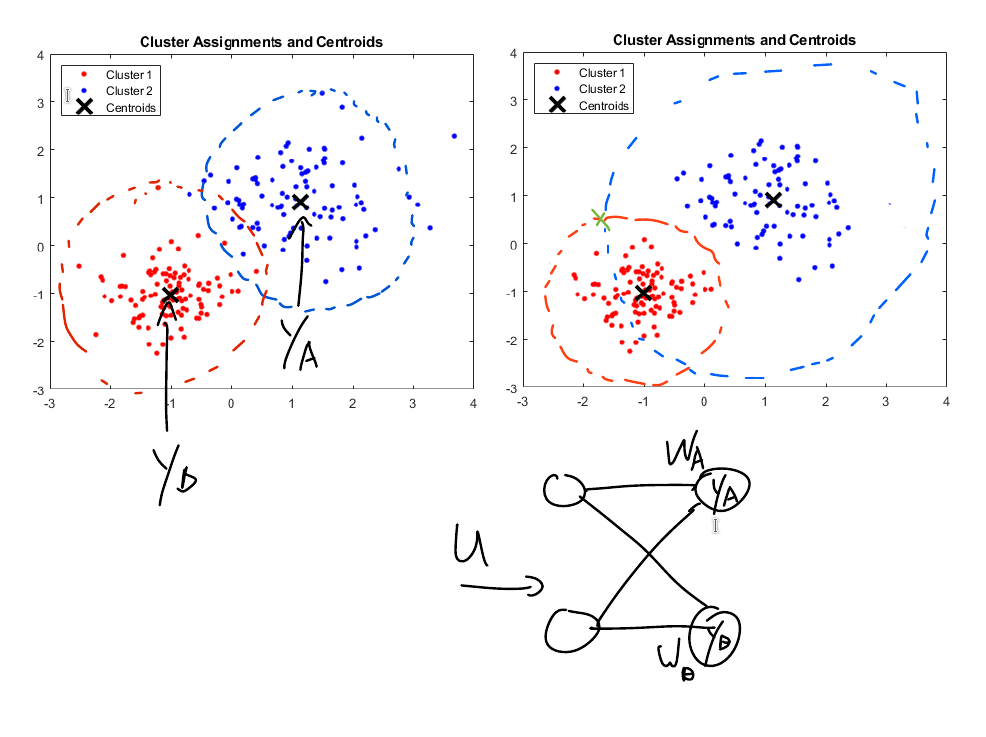
\includegraphics[width=0.8\linewidth]{07_UnsupervisedAndSelfsupervisedLearning/figures/competitive-nn.png}
	\label{fig:competitive-nn}
	\caption{Competitive NN: The position of the two neurons after convergance (left). A new datapoint and the datapoints equidistance line to the cluster-center neurons (right). The network structure(bottom).}
\end{figure}


\subsection{Self Organizing Maps}
 When a training example is fed to the network, its Euclidean distance to all weight vectors is computed. The neuron whose weight vector is most similar to the input is called the best matching unit (BMU). The weights of the BMU and neurons close to it in the SOM grid are adjusted towards the input vector.The magnitude of the change decreases with time and with the grid-distance from the BMU.

\begin{figure}[H]
	\centering
	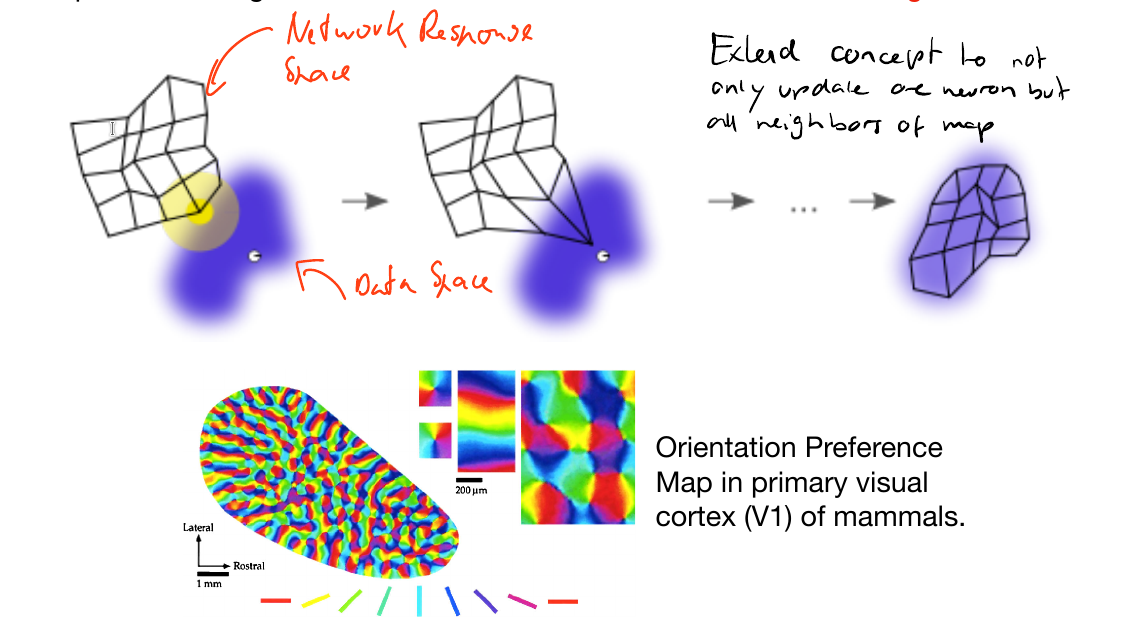
\includegraphics[width=0.9\linewidth]{07_UnsupervisedAndSelfsupervisedLearning/figures/competitive-som.png}
	\label{fig:competitive-som}
	\caption{Self Organizing Map}
\end{figure}


\section{Probabilistic (Generative) UL Methods}
\subsection{Plots of Different Methods}
As a summary:
\begin{figure}[H]
	\centering
	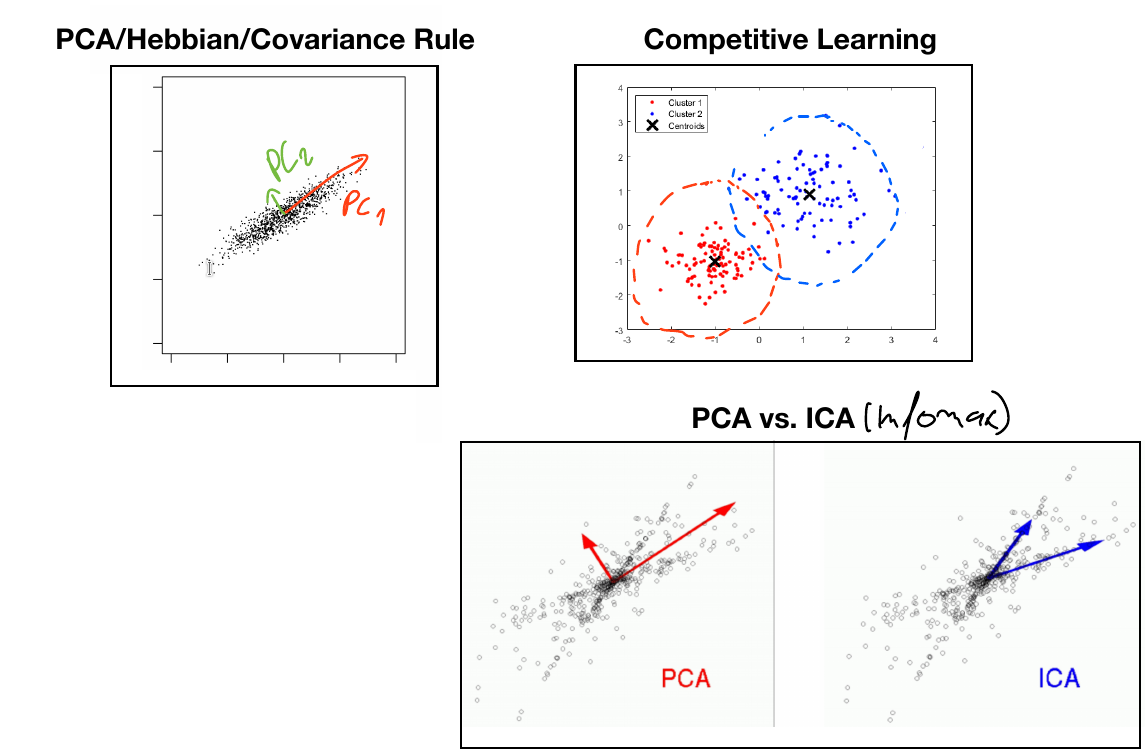
\includegraphics[width=0.9\linewidth]{07_UnsupervisedAndSelfsupervisedLearning/figures/summary-clustering.png}
	\label{fig:summary-clustering}
	\caption{PCA, Competitive Learning and ICA in one picture}
\end{figure}

\subsection{Probabilistic Generative Models}
We know that or data has some causes $v$, but its hard to specify those. We do not know the underlying distribution. We can see the real world as a generative model that produced our (observable) data $u$. Now we want to mimic this process. We model the causes as prior $p(v,G)$ and our generative model specifies the artificial data distribution $p(u|v,G)$. We have a recognition model that maps the samples gathered in the "real" world somehow to our generative model (not clear from the slides how).


Goal: Learn a good generative model that mimics the statistics of the data generation process
Approach: Given data, solve two problems:

\begin{enumerate}
    \item Estimate the causes by computing the posterior
    \item Learn all parameters $G$ of the model and the latent space statistics.
\end{enumerate}

A very basic example is a mixture of Gaussians:

\begin{equation}
    p(u,G) = \sum_v p(u|v,G)p(v,G)
\end{equation}

\begin{equation}
    G = (\mu_v, \tau_v, y_v)
\end{equation}
I assume these parameters are means, variances and mixture scaling factors.

There are several ways how one could use a neural network for these challenges. Also known as ‘Maximum Likelihood Learning’:
\begin{itemize}
    \item Learn the recognition model
    \item Learn the generative model
    \item Learn/update the prior $p(z)$
\end{itemize}

\begin{figure}[H]
	\centering
	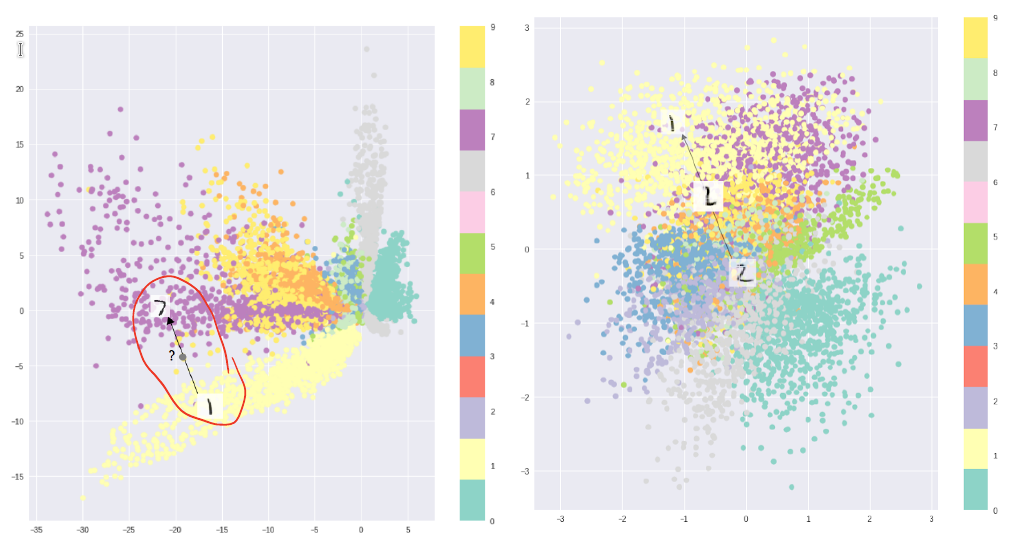
\includegraphics[width=0.9\linewidth]{07_UnsupervisedAndSelfsupervisedLearning/figures/generative-vs-trad-embed.png}
	\label{fig:generative-vs-trad-embed}
	\caption{The difference between an traditional embedding algorithm on the left where we have huge gaps in embedding space and a generative embedding method on the right that densely covers the space. This allows us to sample.}
\end{figure}

\subsection{The restricted Boltzmann Machine}
A restricted Boltzmann machine (RBM) is a generative stochastic artificial neural network that can learn a probability distribution over its set of inputs. As their name implies, RBMs are a variant of Boltzmann machines, with the restriction that their neurons must form a bipartite graph. This means that in restricted Boltzmann machines there are only connections (dependencies) between hidden and visible units, and none between units of the same type (no hidden-hidden, nor visible-visible connections). Although learning is impractical in general Boltzmann machines, it can be made quite efficient for RBMs. A deep Boltzmann machine (DBM) is a type of binary pairwise Markov random field (undirected probabilistic graphical model) with multiple layers of hidden random variables.

Practical details:
\begin{itemize}
    \item RBMS have two biases (visible and hidden).
    \item The hidden bias helps the RBM produce the activations on the forward pass, while
    \item The visible layer’s biases help the RBM learn the reconstructions on the backward pass.
\end{itemize}

\begin{figure}[H]
	\centering
	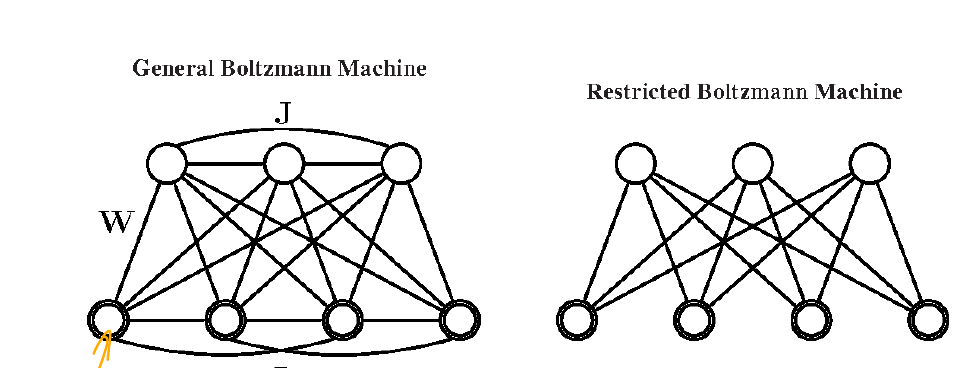
\includegraphics[width=0.9\linewidth]{07_UnsupervisedAndSelfsupervisedLearning/figures/boltzmann-res-ures.png}
	\label{fig:boltzmann-res-ures}
	\caption{Difference between a general and a restricted Boltzmann machine. The weights (orange arrow) are probabilistic units with activation 0 or 1. In Boltzmann machines, information flows forward and backwards.}
\end{figure}
\begin{figure}[H]
	\centering
	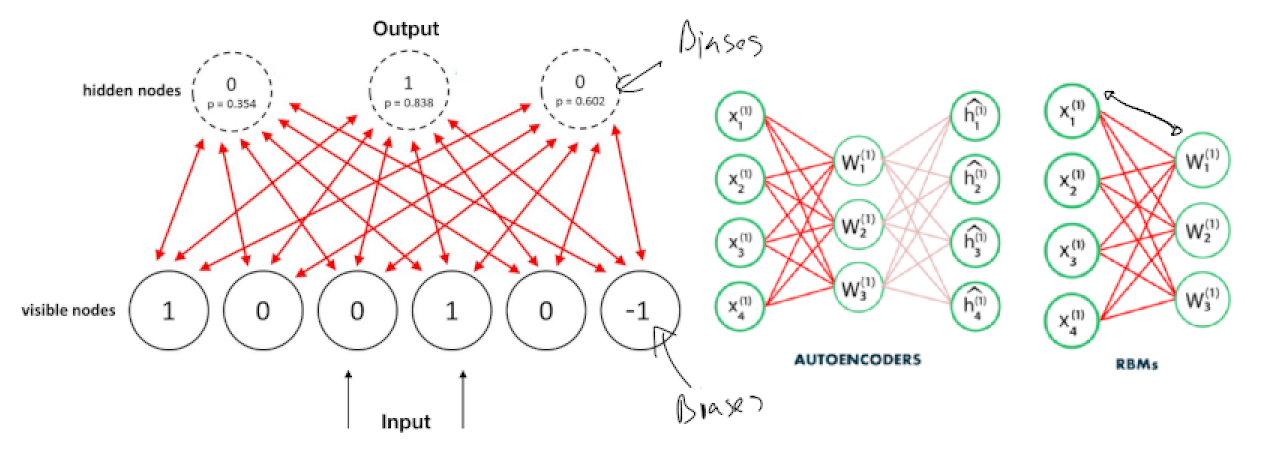
\includegraphics[width=0.9\linewidth]{07_UnsupervisedAndSelfsupervisedLearning/figures/boltzmann-in-action.png}
	\label{fig:boltzmann-in-action}
	\caption{(right) RBMs are similar to (reverse) autoencoders but use stochastic units with particular distribution instead of deterministic distribution. The task of training is to find out how these two sets of variables are connected to each other. (left) The difference between the hidden nodes which are probabilistic and the input nodes.}
\end{figure}

\subsubsection{Training the Restricted Boltzmann Machine (Contrastive Divergence)}
Is not used anymore because back-propagation works so well. Attempts were made to use RBMs as dimensionality reduction algorithm. Results were okay, compared to PCA, the clusters seem more dense and separated.


Training algorithm:
\begin{enumerate}
    \item Take a sample $V_0$ and compute the hidden activation vector $h_0$. Call $V_0 h_0^T$ (outer product) the positive gradient.
    \item Sample from $h_0$, compute $V_1$, resample from $V_1$, compute $h_1$. Call $V_1 h_1^T$ the negative gradient.
    \item Update weights: $\nabla w = \eta (v_0h_0 - v_1h_1)$
\end{enumerate}

\begin{figure}[H]
	\centering
	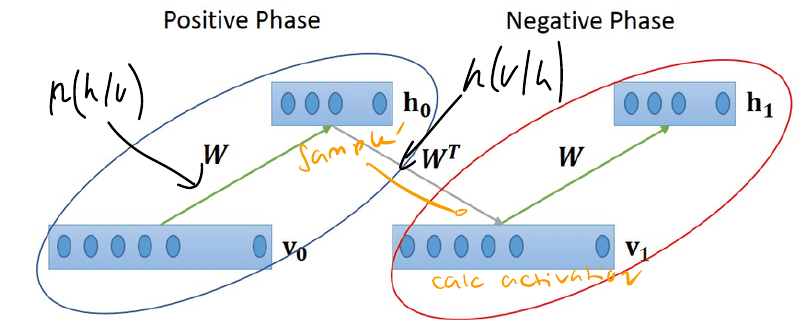
\includegraphics[width=0.9\linewidth]{07_UnsupervisedAndSelfsupervisedLearning/figures/boltzmann-contr-div.png}
	\label{fig:boltzmann-contr-div}
	\caption{Visualization of the training algorithm}
\end{figure}

\subsection{Helmholtz Machines}
\epigraph{"Never really worked"}{Prof. Grewe}

A Helmholtz machine contains two networks, a bottom-up recognition network that takes the data as input and produces a distribution over hidden variables, and a top-down "generative" network that generates values of the hidden variables and the data itself.

Helmholtz machines were created to improve noise resilience, which is always present in natural data, and in hope that by learning economical representations of the data, the underlying structure of the generative model should reasonably approximate the hidden structure of the data set. 

The two phases of the Boltzmann machine contrast the statistics of the activations of the network when input patterns are presented with the statistics of the activations of the network when it is running ‘free’. This contrastive procedure involves substantial noise and is slow. The Helmholtz machine does not have this problem.

\subsubsection{Wake-Sleep Algorithm}
Used to train Helmholtz Machines. The wake and sleep phases are not contrastive. Rather, the recognition and generative models are forced to chase the other.

\begin{itemize}
    \item Wake Phase: \textbf{Use the recognition weights} to perform a bottom up pass and \textbf{train the generative weights} to reconstruct the activity in each layer from the layer above.
    \item Sleep Phase (because the network is insensitive to input): \textbf{Use the generative weights} to generate samples from the model, propagate these from top to bottom and \textbf{then use (train) the recognition weights} to reconstruct the activities in each layer from the layer below.
\end{itemize}
 
 \begin{figure}[H]
	\centering
	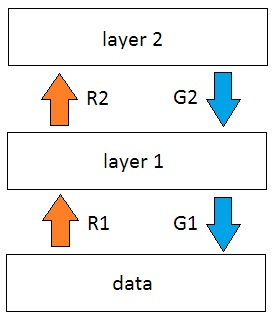
\includegraphics[width=0.3\linewidth]{07_UnsupervisedAndSelfsupervisedLearning/figures/wake-sleep.jpg}
	\label{fig:wake-sleep}
	\caption{Layers of the neural network. R, G are weights used by the wake-sleep algorithm to modify data inside the layers.}
\end{figure}

\subsection{Variational Autoencoders}
The idea of Variational Autoencoder (Kingma \& Welling, 2014), short for VAE, is actually less similar to all the autoencoder models above, but deeply rooted in the methods of variational bayesian and graphical model. Instead of mapping the input into a fixed vector, we want to map it into a distribution. 

 \begin{figure}[H]
	\centering
	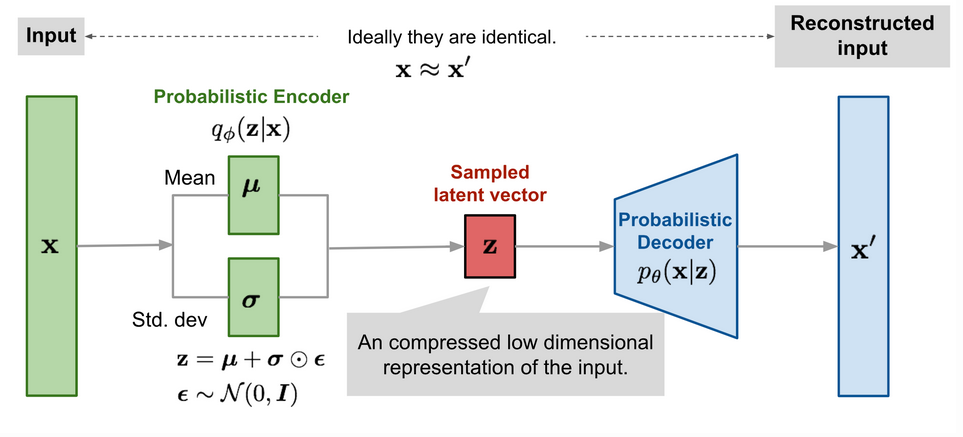
\includegraphics[width=0.9\linewidth]{07_UnsupervisedAndSelfsupervisedLearning/figures/autoencoder-vae.png}
	\label{fig:wake-sleep}
	\caption{Illustration of variational autoencoder model with the multivariate Gaussian assumption.}
\end{figure}

\subsubsection{Reparametrization Trick}
 \begin{figure}[H]
	\centering
	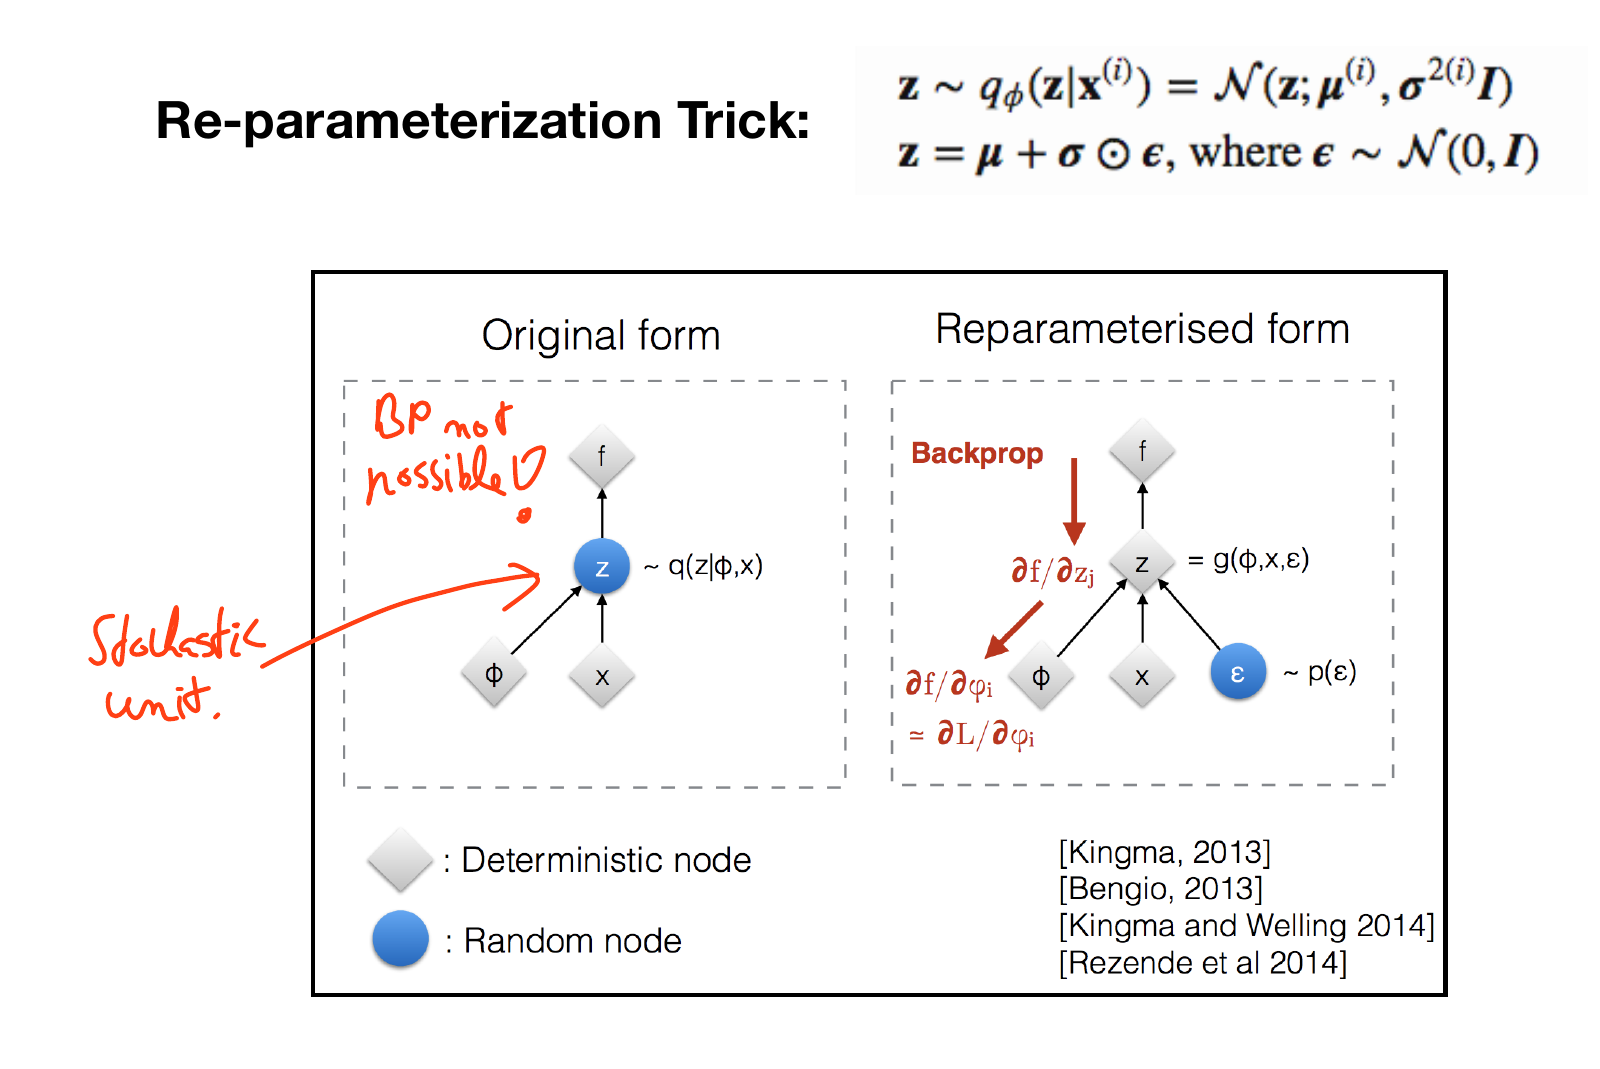
\includegraphics[width=0.9\linewidth]{07_UnsupervisedAndSelfsupervisedLearning/figures/reparam.png}
	\label{fig:reparam}
	\caption{Reparametrization trick in detail.}
\end{figure}

\subsubsection{VAE Loss}
The VAE loss function is an application of the reparametrization trick. It allows to back-propagate from the decoder side to the encoder side. Without this trick, the bottleneck would be fully probabilistic without a chance to compute a gradient flow trough.


\begin{align}
L_\text{VAE}(\theta, \phi) 
&= -\log p_\theta(\mathbf{x}) + D_\text{KL}( q_\phi(\mathbf{z}\vert\mathbf{x}) \| p_\theta(\mathbf{z}\vert\mathbf{x}) )\\
&= - \mathbb{E}_{\mathbf{z} \sim q_\phi(\mathbf{z}\vert\mathbf{x})} \log p_\theta(\mathbf{x}\vert\mathbf{z}) + D_\text{KL}( q_\phi(\mathbf{z}\vert\mathbf{x}) \| p_\theta(\mathbf{z}) ) \\
\theta^{*}, \phi^{*} &= \arg\min_{\theta, \phi} L_\text{VAE}
\end{align}

In Variational Bayesian methods, this loss function is known as the variational lower bound, or evidence lower bound.
Therefore by minimizing the loss, we are maximizing the lower bound of the probability of generating real data samples.

\begin{equation}
    -L_\text{VAE} = \log p_\theta(\mathbf{x}) - D_\text{KL}( q_\phi(\mathbf{z}\vert\mathbf{x}) \| p_\theta(\mathbf{z}\vert\mathbf{x}) ) \leq \log p_\theta(\mathbf{x})
\end{equation}


 \begin{figure}[H]
	\centering
	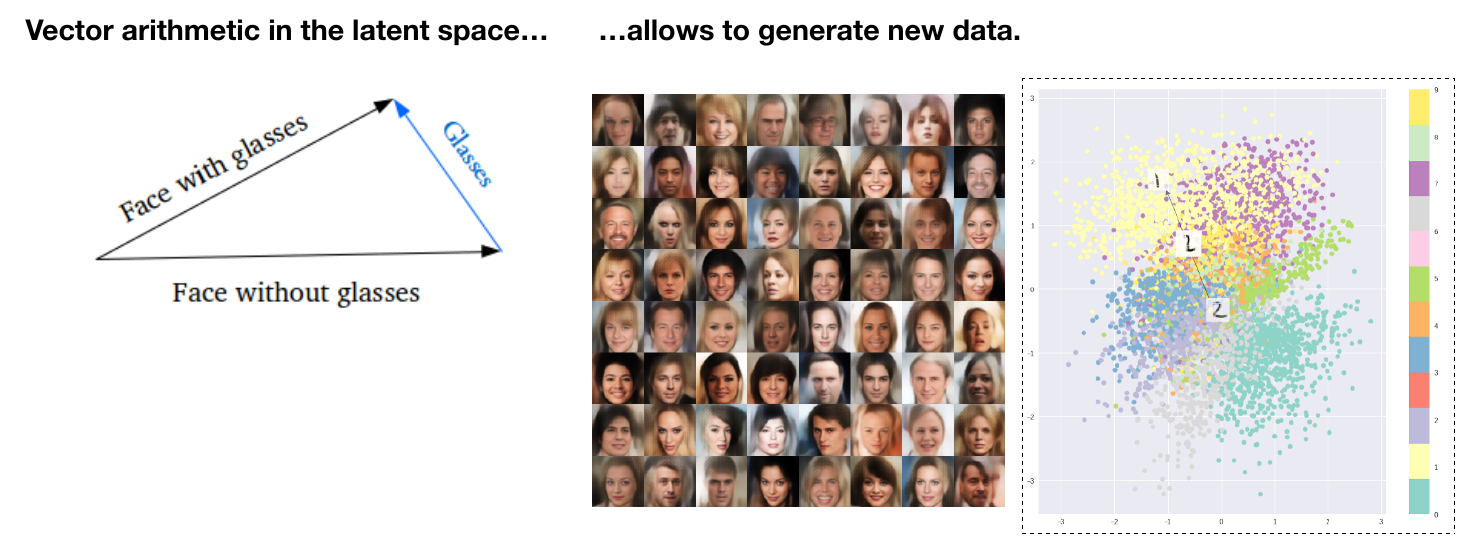
\includegraphics[width=0.9\linewidth]{07_UnsupervisedAndSelfsupervisedLearning/figures/autoencoder-vae-gen.png}
	\label{fig:reparam}
	\caption{We can perform vector arithmetic in the latent space which is densely covered and then use the decoder to map to a sample in data space.}
\end{figure}

\subsection{Predictive Coding}
Predictive coding (also known as predictive processing) is a theory of brain function in which the brain is constantly generating and updating a mental model of the environment. The model is used to generate predictions of sensory input that are compared to actual sensory input. This comparison results in prediction errors that are then used to update and revise the mental model. In short: the brain tries to predict the next input to our network.

 \begin{figure}[H]
	\centering
	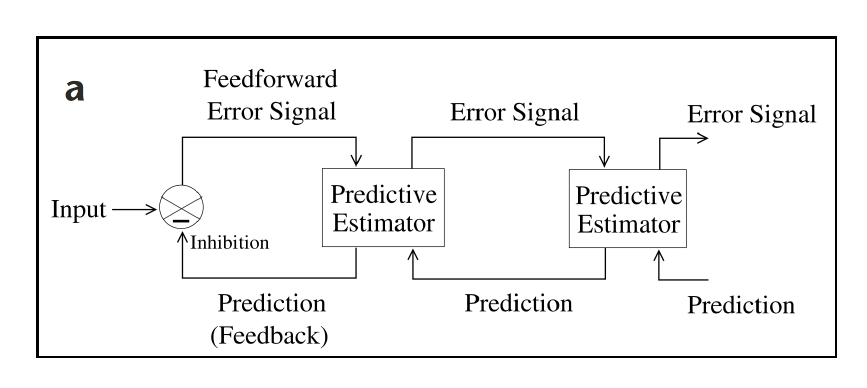
\includegraphics[width=0.9\linewidth]{07_UnsupervisedAndSelfsupervisedLearning/figures/pred-coding-overview.png}
	\label{fig:pred-coding-overview}
	\caption{Inhibiting feedback prediction mechanism in the visual cortex.}
\end{figure}

\subsubsection{Deep Predictive Coding: Pred-Net}
The network consists of a series of repeatingstacked modules that attempt to make local predictions of the input to the module, which is thensubtracted from the actual input and passed along to the next layer. 

 \begin{figure}[H]
	\centering
	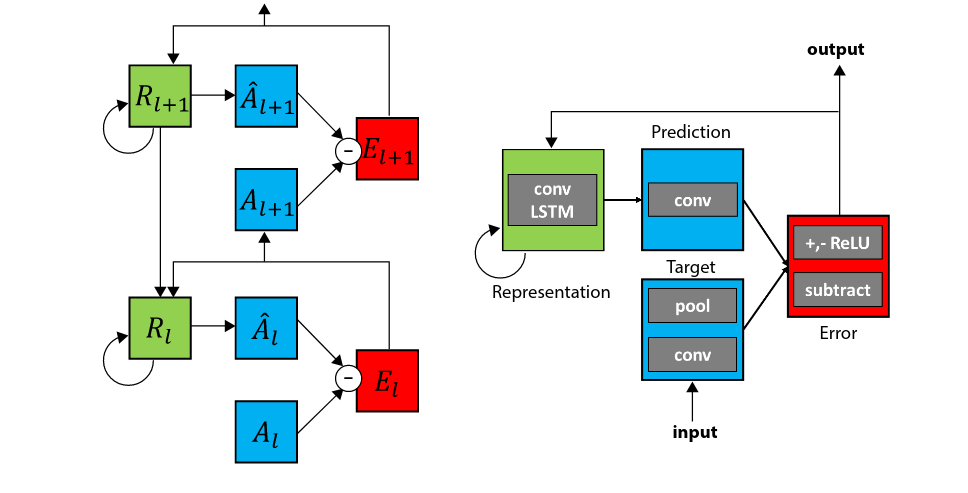
\includegraphics[width=0.9\linewidth]{07_UnsupervisedAndSelfsupervisedLearning/figures/pred-net.png}
	\label{fig:pred-net}
	\caption{Figure 1:  Predictive Coding Network (PredNet).  Left:  Illustration of information flow within two layers. Each layer consists of representation neurons ($R_l$), which output a layer-specific prediction ateach time step ($\hat{A}_l$), which is compared against a target ($A_l$) (Bengio, 2014) to produce an error term($E_l$), which is then propagated laterally and vertically in the network. Right: Module operations forcase of video sequences.}
\end{figure}

 \begin{figure}[H]
	\centering
	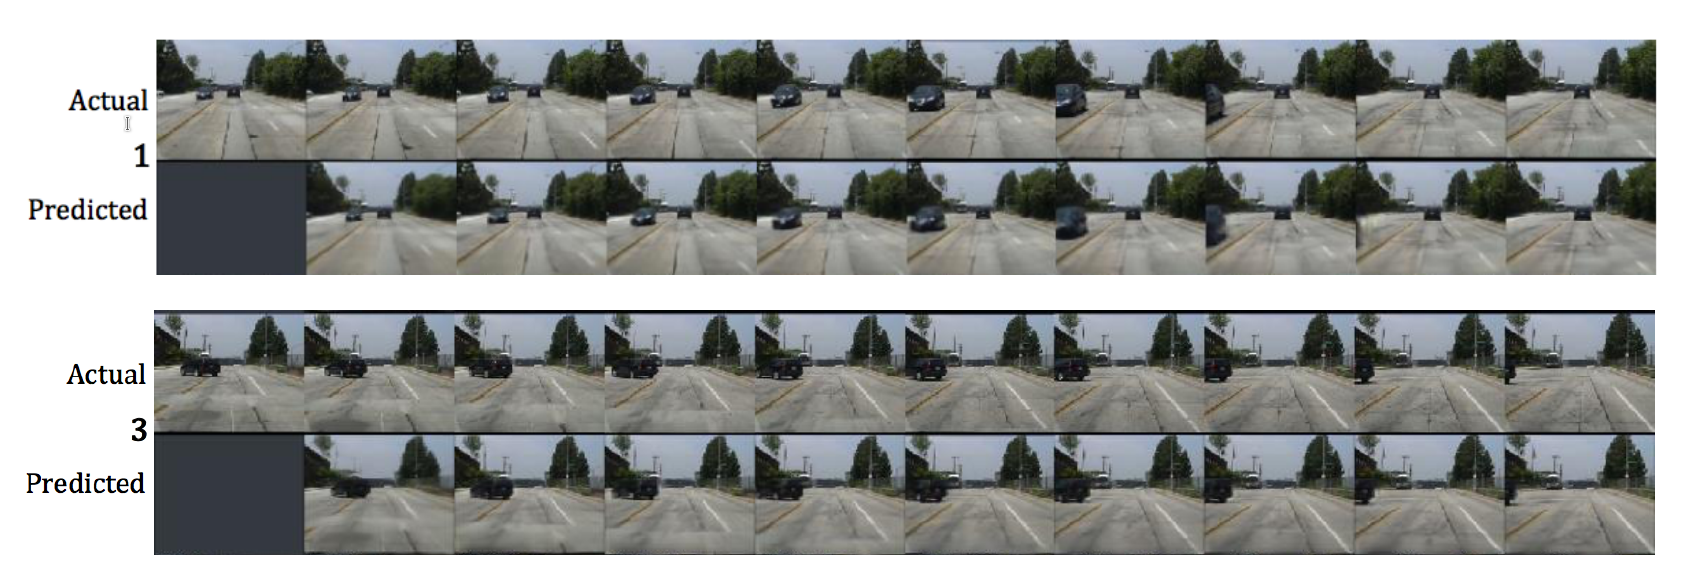
\includegraphics[width=0.9\linewidth]{07_UnsupervisedAndSelfsupervisedLearning/figures/pred-net-out.png}
	\label{fig:pred-net-out}
	\caption{The PredNet in action}
\end{figure}

\subsection{Pixel-RNN}
The PixelRNN is a generative model for images. The network models conditional distribution of every individual
pixel given previous pixels (to the left and to the top).

\begin{equation}
    p(\mathbf{x}) = \prod_{i=1}^{n^2} p(x_i|x_1, ..., x_{i-1})
\end{equation}

 \begin{figure}[H]
	\centering
	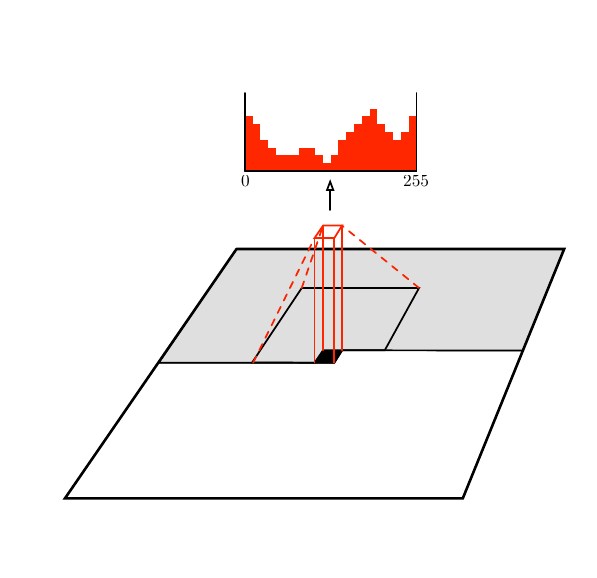
\includegraphics[width=0.5\linewidth]{07_UnsupervisedAndSelfsupervisedLearning/figures/pixel-rnn.png}
	\label{fig:pred-net-out}
	\caption{Distribution over color space of a single pixel in the generative process of the PixelRNN.}
\end{figure}

\subsection{What you should know}

You should be able to explain:
\begin{itemize}
 \item the idea of sparse coding, including formulas.
 \item competitive learning in NNs.
 \item the different concepts of auto encoders and their cost functions.
 \item the Boltzmann machine.
 \item the Helmholtz machine and the wake-sleep algorithm.
 \item the basic idea behind VAEs and the re-parametrization trick.
 \item the idea behind predictive coding and its relation to neuroscience.
 \item the (dis)advantages of generative vs. non-generative UL methods.
\end{itemize}

\end{document}